\documentclass[french,a4paper,12pt]{report}
\documentclass[french,a4paper,12pt]{report}
\usepackage[utf8]{inputenc}
\usepackage[T1]{fontenc}
\usepackage{graphicx}
\usepackage{float}
\usepackage{listings}
\usepackage{color}
\definecolor{dkgreen}{rgb}{0,0.6,0}
\definecolor{gray}{rgb}{0.5,0.5,0.5}
\definecolor{mauve}{rgb}{0.58,0,0.82}

\lstset{frame=tb,
  language=Java,
  aboveskip=3mm,
  belowskip=3mm,
  showstringspaces=false,
  columns=flexible,
  basicstyle={\small\ttfamily},
  numbers=none,
  numberstyle=\tiny\color{gray},
  keywordstyle=\color{blue},
  commentstyle=\color{dkgreen},
  stringstyle=\color{mauve},
  breaklines=true,
  breakatwhitespace=true,
  tabsize=3
}



\title{LO52\\ Travaux Pratiques 5:\\ Introduction à l'AOSP}
\author{Professeur encadrant : \\BRISSET Fabien \\ \\ Elèves : \\ROMET Pierre
\\PROST Guillaume \\ \\ \\}
%\hfill\hbox to 0pt{\hss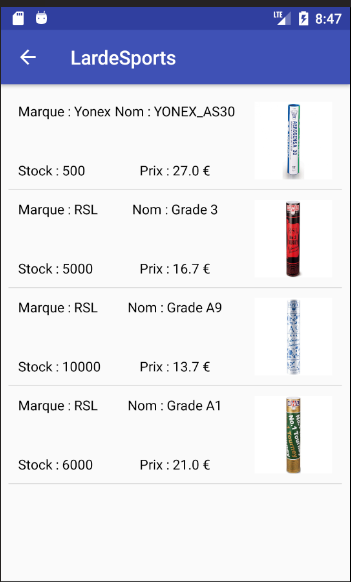
\includegraphics[width=7cm]{Rapport_screen_activity-Stock_liste.png}\hss}\hfill\null\newline
\date{Automne 2017}

\begin{document}

\maketitle
\tableofcontents

\chapter{Objectif}
Dans ce Tp, il nous fut proposé de travailler avec le NDK Android.
Le NDK est un ensemble d'outils, permettant d'implémenter des éléments d'un
projet en utilisant un langage natif, tel que le C et le C++.
Afin de déployer une couche JNI au sein d'une application Android.
Le JNI est un mécanisme de programmation de plus en plus présent sous Android;
permettant de déployer des binding.

\chapter{Interface graphique}
Dans un premier temps, nous avons dû déployer une application Android, avec une
interface composée des éléments suivants;
\begin{itemize}
  \item Un label
  \item Un champ de saisi
  \item Quatre boutons
\end{itemize}

Notre interface se présente donc comme suivant:

\hfill\hbox to 0pt{\hss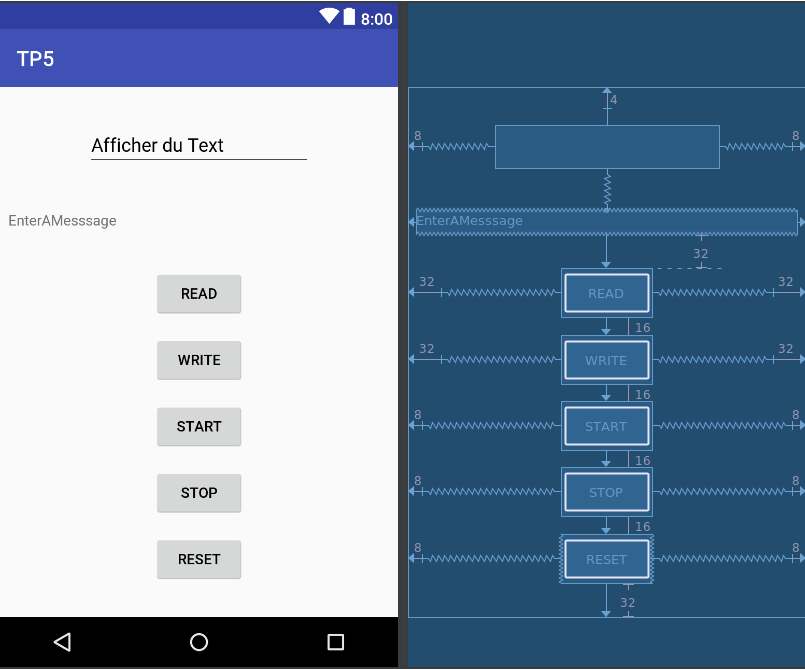
\includegraphics[width=10cm]{1.png}\hss}\hfill\null\newline

\chapter{JNI}

Apèrs avoir créé notre application Android (en spécifant lors de la création,
la prise en compte du paramètre "#include C++ Support"), nous nous sommes tourné vers
l'intégration de la JNI au sein de notre projet.

Pour cela nous avons commencé par déclarer les prototypes des fonctions natives,
(au sein d'une classe C++) que nous devions intégrer, en respectant le standard
de programmation imposé par la JNI.

\section{JNI - Prototype de fonction}

Nous avons déployé cinq fonctions en respectant la norme suivante:

\begin{lstlisting}
  JNIEXPORT <type_retour> JNICALL Java_<package_tree>_<class_name>_<methode_name>
  (JNIEnv * env, jObject this, <TYPE parameter>);
\end{lstlisting}

Ainsi, les prototypes de nos fonctions furent déclarés comme suivant:

\begin{lstlisting}
#include <jni.h>
/*
* Read function
*/
JNIEXPORT jstring JNICALL Java_com_lo52_dewback_tp5_LO52MainActivity_read
(JNIEnv * env, jobject obj, jstring myString)

/*
* Write function
*/
JNIEXPORT jstring JNICALL Java_com_lo52_dewback_tp5_LO52MainActivity_write
(JNIEnv *env, jobject obj, jstring myString)

/*
* Stop function
*/
JNIEXPORT jstring JNICALL Java_com_lo52_dewback_tp5_LO52MainActivity_stop
(JNIEnv *env, jobject obj, jint myInt)

/*
* Start function
*/
JNIEXPORT jstring JNICALL Java_com_lo52_dewback_tp5_LO52MainActivity_start
(JNIEnv *env, jobject obj, jint myInt)

/*
* Reset functionpublic void onReset(View pView)
*/
JNIEXPORT jstring JNICALL Java_com_lo52_dewback_tp5_LO52MainActivity_reset
(JNIEnv *env, jobject obj)
\end{lstlisting}

\section{JNI - Code C++}

Par la suite,
au sein de notre classe Java principale "LO52MainActivity.java", nous avons
utilisé la fonction suivante afin de charger notre bibliothèque JNI.

\begin{lstlisting}
  static {
      System.loadLibrary("native-lib");
  }
\end{lstlisting}

Puis, nous avons initialisé nos cinq fonctions comme suivant; chaque prototype
étant préfixé de l'attribut "Native", qui en java spécifie que la fonction
référence un code natif.

\begin{lstlisting}
  native String read(String pString);
   native String write(String pString);
   native String stop(int pInt);
   native String start(int pInt);
   native String reset();
\end{lstlisting}

Enfin, nous avons défini les fonctions, déclenché par un appui sur l'un des
boutons de notre interface, nous permettant de faire appel à nos fonctions natives.

\begin{lstlisting}
  public void onRead(View pView);
  public void onWrite(View pView);
  public void onStart(View pView);
  public void onStop(View pView);
  public void onReset(View pView);
\end{lstlisting}


\end{document}
